\documentclass[a4paper]{report}
\usepackage{graphicx}
\usepackage{array}
\usepackage{natbib}
\usepackage{hyperref}
\usepackage[english]{babel}
\usepackage{lscape}
\usepackage{longtable}

\begin{document}
\begin{titlepage}
\begin{center}
\textsc{\LARGE Contextproject Programming Life}\\
\vspace{5pt}
\textsc{\LARGE Group 2 - GEVATT}\\
\vspace{5pt}
\textsc{\LARGE Final Report}\\
\vspace{5pt}
\textsc{\large TU Delft}

\begin{table}[ht]
\centering
\begin{tabular}{ccc}

\includegraphics[scale=0.2]{ruben.png}   &

\includegraphics[scale=0.2]{mathijs.png} &

\includegraphics[scale=0.2]{jasper.png}  \\
Ruben Bes	& Mathijs Hoogland	& Jasper Denkers\\
rbes 		& mhhoogland 		& jdenkers\\
4227492 	& 4237676 			& 4212584\\
\end{tabular}
\end{table}

\begin{table}[ht]
\centering
\begin{tabular}{cc}
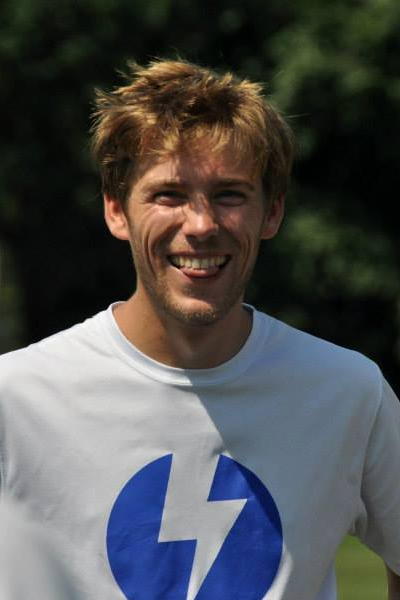
\includegraphics[scale=0.2]{robbert.png} &

\includegraphics[scale=0.2]{willem.png}  \\
Robbert van Staveren	& Willem Jan Glerum\\
rhvanstaveren 			& wglerum\\
1527118					& 4141040\\
\end{tabular}
\end{table}

\vfill
{\large \today}
\end{center}

\end{titlepage}

\begin{landscape}
\setlength\extrarowheight{5pt}
\begin{longtable}{p{3cm}|p{3cm}|p{1cm}|p{2cm}|l|l|p{5cm}}

\textbf{Story} & \textbf{Task} & \textbf{Effort} & \textbf{Assignment} & \textbf{Actual effort} & \textbf{Done} & \textbf{Notes}\\
\hline \hline

A user wants to have an overview of mutations per patient 
& Look up homozygote SNPs & 6 & Mathijs \& Ruben & 10 hours & Yes & Done. Took some time to figure out how to get other kind of information. \\
& Show relevant information per chromosome in overview visualization & 6 & Mathijs & 5 hours & Yes & There's a separate overview per chromosome now. \\
& Implement the XY/XX chromo- some & 10 & Mathijs & 10 hours & Done & Mathijs implemented the functionality. Option added in form for adding a patient to indicate if the patient is male or female.\\
\hline

A user wants to view links between genes and proteins related to a mutation 
& Show multiple mutations per graph & 6 & Robbert \&Jasper & 10 hours & Yes & Quite hard to get information quickly. Finally made the processing of finding related mutations based on proteins after uploading a file. Connections are saved in the database so viewing the graphs stays quick. \\
\hline

A user looks at an overview of the location of a mutation & Look if other genes are near the starting point of a mutation & 6 & Willem Jan & 12 hours & Yes & Willem Jan updated the whole visualisation with 20 genes and there locations indicated by horizontal bars. \\
& Show neighbouring mutations & 6 & Willem Jan & 5 hours & Yes & See previous point. \\
\hline

Database testing 
& Give proper errors when database fails & 4 & - & - & No & Skipped this due to time considerations. \\
\hline

A user logs in and views basic information 
& Optimize dashboard information & 2 & Jasper & 4 hours & Yes & Done, removed unused pages and merged to the dashboard. Dashboard got an update. \\
\hline

For future changes, programmers must not have a hard time under- standing and changing code
& Splitting long functions & 3 & Robbert & 5 hours & Yes & Improved code structure by splitting too long functions (mainly database related). \\
& Checkstyle & 4 & All & 4 hours & Yes & Improved, almost everything covered now. \\
& JavaDoc & 2 & All & 3 hours & Yes & Made code more readable. \\
& Tests & 5 & All & 10 hours & Yes & Adjusted tests of changed code and added to increase coverage. \\
\hline

Deliverables
& Scrum reflection 5 week 9 & 2 & Jasper & 1 hour & Yes & None.\\
& Final Report Draft & 5 & Jasper \& Mathijs \& Willem Jan & 15 hours & Yes & Mathijs did HCI chapter, Willem Jan evaluation. Jasper made other chapters and putter things together. \\
& Architecture Design Draft 2 & 5 & Ruben & 5 hours & Yes & Most of feedback was already processed. \\
\hline
\end{longtable}
\end{landscape}

\section*{General Reflection}
Last week with a lot of finishing touches. Some little extra features were added like background processing of the VCF files. All visualisations are finished and we have a working product. Still some minor issues with database connections but managed to get it working.

All of us are working well with branches and this improved our workflow. No more wrong code in master and each separate part was developed in a separate branch. We dropped the part of giving proper database errors but still, by good planning, were ably to get everything done in time.

Final report just took some time but was made. EAD had a bit less work because some earlier feedback was already processed. \\
\end{document}